\section{Dilation and erosion}
One must employ care when using the morphological operators dilation and erosion. As they are not inverses of each other, the effect of applying one and then the other is not the same as applying them in reverse order. An example of this can be seen in \autoref{dilationErosion}. In the example we also see the advantage of erosion and dilation as the figure is now closed, i.e. we removed the hole.

\begin{figure}[h]
	\centering
	\begin{subfigure}{0.3\linewidth}
		\centering
		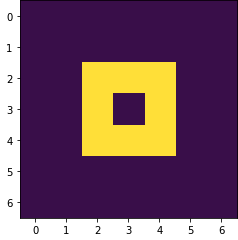
\includegraphics[width=\linewidth]{Materials/morphOrg}
		\caption{Original image.\newline}
	\end{subfigure}
	\hfill
	\begin{subfigure}{0.3\linewidth}
		\centering
		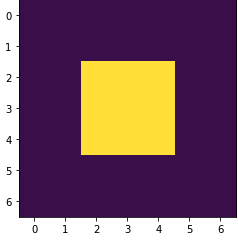
\includegraphics[width=\linewidth]{Materials/morphDilation}
		\caption{Original image after dilation and then erosion.}
	\end{subfigure}
	\hfill
	\begin{subfigure}{0.3\linewidth}
		\centering
		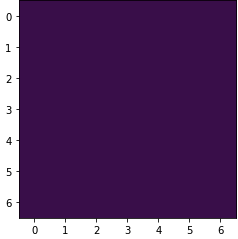
\includegraphics[width=\linewidth]{Materials/morphErosion}
		\caption{Original image after erosion and then dilation.}
	\end{subfigure}
	\caption{Example of applying dilation and then erosion is not the same as applying erosion and then dilation.}
	\label{dilationErosion}
\end{figure}
In a real scenario one might want to close holes in an initial segmentation of microvasculature (\autoref{microvasculature}) or in a brain (\autoref{brain}), but if one uses erosion on the microvasculature they risk disconnecting the vessels or even worse removing tips of the vessels. In the brain segmentation if dilation is used one risks the brain folds collapse and the brain becoming one big blob. Thus, care must be taken when segmenting thin objects not to make erosions, and care must be taken not to make dilations when details in a segmentation spatially lie very close to other details in the segmentation. However, when care \textit{is} taken, one can close the holes and remove leaks from their segmentation using dilation and erosion, and thus obtain an improved segmentation.

\begin{figure}[h]
	\centering
	\begin{subfigure}{0.3\linewidth}
		\centering
		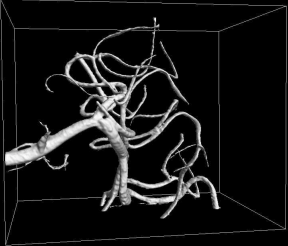
\includegraphics[width=\linewidth]{Materials/microvasculature}
		\caption{Initial segmentation of microvasculature.}
		\label{microvasculature}
	\end{subfigure}
	\hspace{1cm}
	\begin{subfigure}{0.3\linewidth}
		\centering
		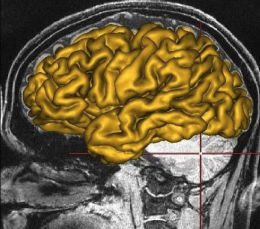
\includegraphics[width=\linewidth]{Materials/brain}
		\caption{Initial segmentation of a brain.}
		\label{brain}
	\end{subfigure}
	\caption{Examples of where care must be taken with dilation and erosion. Images taken from slides.}
\end{figure}